%\emph{•}%%%%%%%%%%%%%%%%%%%%%%%%%%%%%%%%%%%%%%%%%
% Short Sectioned Assignment
% LaTeX Template
% Version 1.0 (5/5/12)
%
% This template has been downloaded from:
% http://www.LaTeXTemplates.com
%
% Original author:
% Frits Wenneker (http://www.howtotex.com)
%
% License:
% CC BY-NC-SA 3.0 (http://creativecommons.org/licenses/by-nc-sa/3.0/)
%
%%%%%%%%%%%%%%%%%%%%%%%%%%%%%%%%%%%%%%%%%
%----------------------------------------------------------------------------------------
%	PACKAGES AND OTHER DOCUMENT CONFIGURATIONS
%----------------------------------------------------------------------------------------
\documentclass[norsk]{article} % A4 paper and 11pt font size

\usepackage[T1]{fontenc} % Use 8-bit encoding that has 256 glyphs
\usepackage{fourier} % Use the Adobe Utopia font for the document - comment this line to return to the LaTeX default
\usepackage[english]{babel} % English language/hyphenation
\usepackage{amsmath,amsfonts,amsthm} % Math packages

% Added by Haavard %---------------------------------------------------------------------
\usepackage[utf8]{inputenc} % Norwegian letters
\usepackage{fullpage}
\usepackage{subcaption}
\usepackage[font={small, it}]{caption} % captions on figures and tables
\usepackage{graphicx}
\usepackage{color}
\usepackage{hyperref} % Use \autoref{ and \nameref{
\hypersetup{backref,
  colorlinks=true,
  breaklinks=true,
  %hidelinks, %uncomment to make links black
  linkcolor=blue,
  urlcolor=blue,
  citecolor=blue
}
\usepackage[all]{hypcap} % Makes hyperref jup to top of pictures and tables
% --------------------------------------------------------------------------------------
% Added by Jorgen %--------------------------------------------------------------------
\usepackage{enumitem} %specifying extra stuff about enumerate
\usepackage{multirow} %For using subrows in tables

% Added by Jorgen, for source code listing %-------------------------------------------
\usepackage{wrapfig}

\usepackage{listings}
\usepackage{xcolor}
\newcommand{\textcolordummy}[2]{#2}

\definecolor{mygray}{rgb}{0.4,0.4,0.4}
%\definecolor{mycyan}{rgb}{0,0.8,0.6}
\definecolor{mygreen1}{rgb}{0.3,0.6,0.3}
\definecolor{mygreen2}{rgb}{0,0.4,0.1}
\definecolor{myorange}{rgb}{1.0,0.4,0}

\lstset{language=C++,
                basicstyle={\color{black}\footnotesize\ttfamily\let\textcolor\textcolordummy},
                %identifierstyle=\color{green},
                keywordstyle={\color{blue}\footnotesize\ttfamily\let\textcolor\textcolordummy},
                %keywordstyle={\color{blue}\footnotesize\ttfamily\let\textcolor\textcolordummy},
                directivestyle={\color{mygreen1}},
                emph={int,char,double,float,unsigned},
                emphstyle={\color{mygreen2}},
                %
                stringstyle={\color{myorange}\footnotesize\ttfamily\let\textcolor\textcolordummy},
                %stringstyle={\color{orange}\footnotesize\ttfamily\let\textcolor\textcolordummy},
                commentstyle={\color{mygray}\footnotesize\ttfamily\let\textcolor\textcolordummy},
                morecomment=[l][\color{magenta}]{\#}
                %
                showspaces=false,  
                showstringspaces=false, 
                showtabs=false,
                extendedchars=true,
                frame=single,  
}
\lstdefinestyle{FormattedNumber}{%
    literate={0}{{\textcolor{red}{0}}}{1}%
             {1}{{\textcolor{red}{1}}}{1}%
             {2}{{\textcolor{red}{2}}}{1}%
             {3}{{\textcolor{red}{3}}}{1}%
             {4}{{\textcolor{red}{4}}}{1}%
             {5}{{\textcolor{red}{5}}}{1}%
             {6}{{\textcolor{red}{6}}}{1}%
             {7}{{\textcolor{red}{7}}}{1}%
             {8}{{\textcolor{red}{8}}}{1}%
             {9}{{\textcolor{red}{9}}}{1}%
             {.0}{{\textcolor{red}{.0}}}{2}% Following is to ensure that only periods
             {.1}{{\textcolor{red}{.1}}}{2}% followed by a digit are changed.
             {.2}{{\textcolor{red}{.2}}}{2}%
             {.3}{{\textcolor{red}{.3}}}{2}%
             {.4}{{\textcolor{red}{.4}}}{2}%
             {.5}{{\textcolor{red}{.5}}}{2}%
             {.6}{{\textcolor{red}{.6}}}{2}%
             {.7}{{\textcolor{red}{.7}}}{2}%
             {.8}{{\textcolor{red}{.8}}}{2}%
             {.9}{{\textcolor{red}{.9}}}{2}%
             ,
   basicstyle=\footnotesize\ttfamily,%  Optional to use this
}

%---------------------------------------------------------------------

\usepackage{lipsum} % Used for inserting dummy 'Lorem ipsum' text into the template

\usepackage{sectsty} % Allows customizing section commands
\allsectionsfont{\centering \normalfont\scshape} % Make all sections centered, the default font and small caps

\usepackage{fancyhdr} % Custom headers and footers
\pagestyle{fancyplain} % Makes all pages in the document conform to the custom headers and footers
\fancyhead{} % No page header - if you want one, create it in the same way as the footers below
\fancyfoot[L]{} % Empty left footer
\fancyfoot[C]{} % Empty center footer
\fancyfoot[R]{\thepage} % Page numbering for right footer
\renewcommand{\headrulewidth}{0pt} % Remove header underlines
\renewcommand{\footrulewidth}{0pt} % Remove footer underlines
\setlength{\headheight}{13.6pt} % Customize the height of the header

\numberwithin{equation}{section} % Number equations within sections (i.e. 1.1, 1.2, 2.1, 2.2 instead of 1, 2, 3, 4)
\numberwithin{figure}{section} % Number figures within sections (i.e. 1.1, 1.2, 2.1, 2.2 instead of 1, 2, 3, 4)
\numberwithin{table}{section} % Number tables within sections (i.e. 1.1, 1.2, 2.1, 2.2 instead of 1, 2, 3, 4)

\setlength\parindent{0pt} % Removes all indentation from paragraphs - comment this line for an assignment with lots of text

%----------------------------------------------------------------------------------------
%	TITLE SECTION
%----------------------------------------------------------------------------------------

\newcommand{\horrule}[1]{\rule{\linewidth}{#1}} % Create horizontal rule command with 1 argument of height

%\title{	
%\normalfont \normalsize 
%\textsc{NTNU} \\ [25pt] % Your university, school and/or department name(s)
%\horrule{0.5pt} \\[0.4cm] % Thin top horizontal rule
%\huge C++  Notes \\ % The assignment title
%\horrule{2pt} \\[0.5cm] % Thick bottom horizontal rule
%}

%\author{Jørgen Vågan} % Your name

%\date{\normalsize\today} % Today's date or a custom date

\begin{document} %---------------------------------------

%\maketitle % Print the title

\section{Tidligere Notater}
To unzip a ''.tgz''-file in linux:
\begin{lstlisting}[style=FormattedNumber, frame=none,language=bash]
   tar xvfz path/file.tgz
\end{lstlisting}
%
For å lese linux filer:
\begin{lstlisting}[style=FormattedNumber, frame=none,language=bash]
   less text.txt
\end{lstlisting}
(q for quit/å avslutte). 
%
For å lage en peker til en executable i en annen mappe (skapt til bruk i hvilken som helst annen mappe), skriv
\begin{lstlisting}[style=FormattedNumber,frame=none, language=bash]
   ln -s RelativePath/yourExecutable .
\end{lstlisting}
For eksempel med \textsc{GranFilm}:
\begin{lstlisting}[style=FormattedNumber,frame=none, language=bash]
   ln -s ../Src/GranFilm .
\end{lstlisting}
For å kjøre \textsc{GranFilm}:
\begin{lstlisting}[style=FormattedNumber,frame=none, language=bash]
   ./GranFilm -p inputParameters.sif -o outputFile.dat
\end{lstlisting}
%
A simple easy plotting program is \textsc{xmgrace}. I think this assumes
data with x-axis at column 1 and everything else on the other columns. Run by typing:
\begin{lstlisting}[style=FormattedNumber,frame=none, language=bash]
   xmgrace dataFile.dat
\end{lstlisting}
or (if you want to plot all the data in the file)
\begin{lstlisting}[style=FormattedNumber,frame=none, language=bash]
   xmgrace -nxy dataFile.dat
\end{lstlisting}


\newpage
\section{Oppsumering Møte 30.April}
\subsection{Plotting med \textsc{Python}}
For å lese filer med pyton er det best å bruke \texttt{numpy.loadtxt(file.dat)}.


\subsection{Truncation Ratio}
%
\begin{figure}[h!]
  \centering
   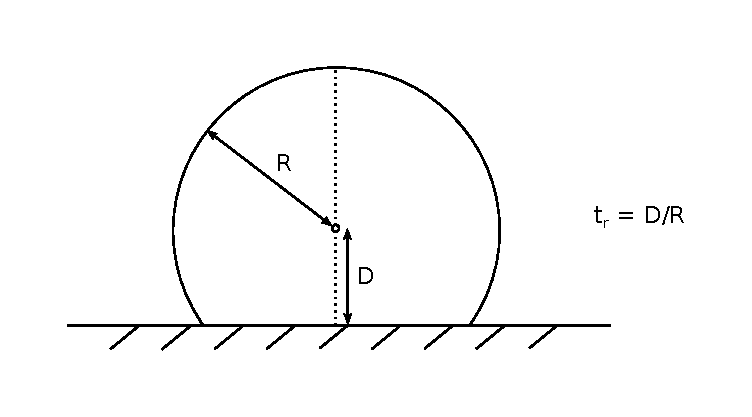
\includegraphics[width=0.5\textwidth]{truncationRatio.pdf}
   \caption{
   The geometrical meaning of the truncation ratio.
   }
   \label{fig:energyComparison}
\end{figure}
%


\subsection{Running Granfilm with -py option}
Skriv 
\begin{lstlisting}[style=FormattedNumber, language=bash]
./GranFilm
\end{lstlisting}
for å se hvilke parametere/flag du kan kjøre prøgrammet med.
\\
\\
Ved å bruk flagget \texttt{-py}, e.g.:
\begin{lstlisting}[style=FormattedNumber, language=bash]
./GranFilm  -py  -p parameters.sif -o output.dat
\end{lstlisting}
får man ekstra ''output''-filer, blant annet \texttt{output.dat\_RefTrans}, se Tabell \ref{tab1}.
%
\begin{table}[htbp]
   \caption{Eksempel på ekstra output data output.dat\_Ref. Fresnel dataen er 
   hva refleksjons koeffisienten er hvis substratet hadde vært bart (flatt, uten dråper)}
\centering
\begin{tabular}{ c c c c }
\hline
 \multicolumn{2}{c}{r\_p}         &  \multicolumn{2}{c}{r\_p fresnel} \\
\hline
$\Re$\{r\_p\}  &  $\Im$\{r\_p\} & $\Re$\{r\_p fresnel\}   & $\Im$\{r\_p fresnel\}  \\
$\downarrow$ & $\downarrow$ &  $\downarrow$         &    $\downarrow$ \\
            &              &              &              \\
\hline
\end{tabular}
\label{tab1}
\end{table}
%

\newpage
\section{Oppsummering Møte 1.Mai}

\subsection{Mål med oppgaven}
Ha termochromst materiale som coating, enten som granular layer eller som coating utenpå et metallisk 
granular layer. Dette skal kunne ''smøres'' på en byggning/vinduer/el. slik at f.eks varmestrålingen 
slippes inn om vinteren når det er kalt ute og reflekteres om sommeren når det er varmt ute.
\\
\\
Om denne optiske endringen kan oppnår ved temperaturgradienten for sommer/vinter kan man unngå bruk av aktive
løsninger (e.g. bruke spenning for å oppnå tilsvarende optiske egenskaper). Materialene burde også
være billig, slik at dette er realiserbart for storskala-prosjekter som store byggninger.
%
\begin{table}[htbp]
   \caption{oppbyggningen av ''.nk'' filene i Sopra-Databasen}
\centering
\begin{tabular}{ c c c c c }
\hline
 \multicolumn{2}{c}{unit}         &  startverdi  &  sluttverdi & antall datapunkter \\
\hline
1          & 2                    &                 &                  & \\
energi[eV] & bølgelengde[$\mu$m]  &  x1[eV/$\mu$m]  &    x2[eV/$\mu$m] & N \\
\hline
\end{tabular}
\label{tab:idealTCW}
\end{table}
%

Så ''.nk-files'' vil være på følgende form:
\begin{lstlisting}[style=FormattedNumber, language=python]
unit		x1			x2	   N	
     n(x1)          k(x1) 
     n(x2)          k(x2) 
     n(x3)          k(x3) 
     n(x4)          k(x4) 
     n(x5)          k(x5) 
     n(x6)          k(x6) 
     n(x7)          k(x7) 
     n(x8)          k(x8) 
     n(x9)          k(x9) 
     n(x10)         k(x10) 
     n(x11)         k(x11) 
     .              .
     .              .
     .              .
\end{lstlisting}
Eksempel: ''mgo.nk'' i eV, startverdi: $0.65$eV, sluttverdi: $10$eV og består av totalt
400 datapunkter:
\begin{lstlisting}[style=FormattedNumber, language=python]
1		0.65			10		400
     1.70969699     0.00000011
     1.71065583     0.00000011
     1.71155117     0.00000011
     1.71239613     0.00000011
     1.71313635     0.00000011
     .              .
     .              .
     .              .
\end{lstlisting}


\subsection{Videre arbeid med oppgaven}
\begin{itemize}
\item Jeg skal finne data på thermochrome dielectrisitetskonstanter og laga en database basert på dette.
   Dette skal bli matet inn i \textsc{GranFilm}.
\item Output burde kanskje være konturplot (for å lettere lese av verdiene, ihvertfall sammenlignet med 3D-plot)
\item Les artikler og finn ''teori'' for å beskrive $\varepsilon(\omega, T)$, men hovedsakelig for å
finne data for $\varepsilon(\omega, T)$.
\end{itemize}

\newpage
\section{Oppsumering E-post 11. Juli}
\begin{itemize}
\item
Anngående dielektriske data: min forståelse av dataen i .nk-fila er riktig.
MEN(!), dataen må være ekvidistansert og helst som kompleks brytningsindex $\hat{n}=n+i\kappa$.
HUSK OGSÅ(!), at n,k-verdier i hver linje i ''.nk'' filen svarer til samme x-verdi.
Jeg må også være oppmerksom på at det finnes to konvensjoner for
tidsavhenigheten til kompleks brytningsindex:
\begin{align}
   e^{-i\omega t}  \:\:\:\:\:\:\:\:\: \text{ og }  \:\:\:\:\:\:\:\:\: e^{+i\omega t} 
\end{align}
Vi bruker førstenevnte (ift. \textsc{GranFilm}), som betyr at positiv
imaginærdel til epsilon betyr absorpsjon ($\Im\{\varepsilon\}>0$). 
(\textit{?er dette påkverd for at det skal være fysisk, type: ingen materialer avgir energy?}).
Jeg må derfor passe på at dataen jeg konverterer har riktig fortegnskonvensjon (elektroingeniører
bruker typisk motsatt av oss).

\item
Kompleks brytningsindeks $\hat{n}=n+i\kappa$ for et ikke magnetisk materiale er definert via
\begin{align}
   \hat{n} = \sqrt{\hat{\varepsilon}(\omega)}, \:\:\:\:\: \text{with Im}\{\hat{n}\} = \kappa > 0,
\end{align}
med vår fortegnskonvensjon.

\item I oppgaven burde jeg klare å lese inn dielektriske data for noen termokromme materialer
   for ulike temperatuerer, samt regne ut hvordan refleksjons egenskapene endrer seg med 
   temperatur i det interessante området ved hjelp av \textsc{GranFilm}.
   Jeg må også diskutere hva disse resultatene betyr.
   \\
   \\
   I tillegg til de eksperimentelle dataene, kan det muligens være av interesse å
   bruke modeller for $\varepsilon(\omega, T)$ om jeg klarer å finne en slik model.
\end{itemize}

\newpage
\section{Oppsummering E-post 5. August}
\subsection{Diverse}
\begin{itemize}
   \item Ift. ''.nk''-filen for luft er $\varepsilon(\omega)=1,\:\: \forall \: \omega$, og kan derfor brukes sammen med 
      annen data uansett energi/bølgelengde intervall.
      \\
      \\
      SiO$_2$ derimot, er svakt dispersiv og kan bare brukes med annen data i det overlappende intervallet.
      Altså, dette er et problem for simuleringer i intervaller der data for en eller flere materialer
      mangler.

   \item For å finne hvor feilmeldinger i programmet kommer i fra, kan feilmeldingen søkes opp
      via:
\begin{lstlisting}[style=FormattedNumber,frame=none, language=bash]
~/Fortran/Projects/Scattering2D/GranFilm/HG/Src tux => grep -in "too few points to spline" *.f90
\end{lstlisting}
\begin{lstlisting}[style=FormattedNumber,frame=none, language=bash]
      SFL_Interpolation.f90:437:    write(*,*) 'too few points to spline'
\end{lstlisting}
(I dette tilfellet var \texttt{'too few points to spline'} feilmeldingen).

\end{itemize}

\subsection{Plasmoner}
\begin{itemize}
   \item Peakene i''polarizability'' størrelsene $\alpha_{\perp}$ og $\alpha_{\parallel}$ er resonanser, og noen av dem er
      ''localized surface plasmons'' (som er dipol resonanser); Andre resonanser er quadrupole resonanser etc...
   \item I tilfellet av en granulær overflate blir både bulk- og overflate-plasmoner eksitert.
   \item ''Localized surface plasmons'' ikke kan eksiteres på en plan overflate. Metallpartikler, som
      er så små at den aktuelle frekvensen får et felt inne i partikkelen, altså at størrelsen på partiklen ikke er større
      enn typisk skinndybde for frekvensen, kan derimot skape localized surface plasmons.
   \item ''The choice of reference Fresnel surface''/''choice of separation surface'' i \textsc{GranFilm}-artikkelen handler bare om
      valg av referansesystem/coordinatsystem.

\end{itemize}

%\begin{lstlisting}[style=FormattedNumber,frame=none, language=bash]
%\end{lstlisting}
%%
%\begin{figure}[h!]
  %\centering
   %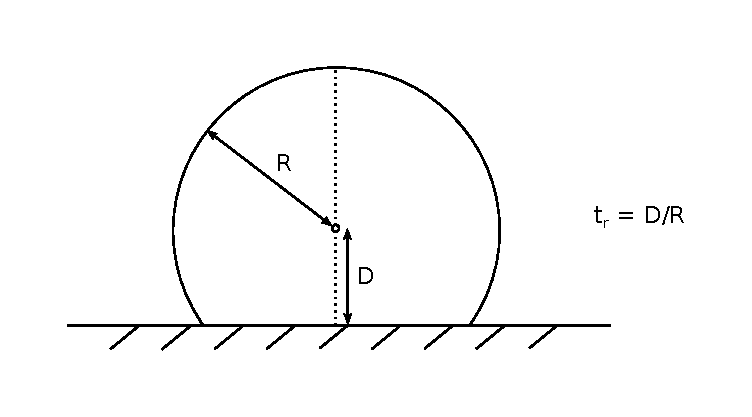
\includegraphics[width=0.5\textwidth]{truncationRatio.pdf}
   %\caption{
   %The geometrical meaning of the truncation ratio.
   %}
   %\label{fig:energyComparison}
%\end{figure}
%%
%\begin{table}[htbp]
   %\caption{oppbyggningen av ''.nk'' filene i Sopra-Databasen}
%\centering
%\begin{tabular}{ c c c c c }
%\hline
 %\multicolumn{2}{c}{unit}         &  startverdi  &  sluttverdi & antall datapunkter \\
%\hline
%1          & 2                    &                 &                  & \\
%energi[eV] & bølgelengde[$\mu$m]  &  x1[eV/$\mu$m]  &    x2[eV/$\mu$m] & N \\
%\hline
%\end{tabular}
%\label{tab:idealTCW}
%\end{table}
%%





%
\end{document}



